\section{TextWorld}
\label{textworld}

TextWorld~\citep{cote2019textworld} is a text-based game environment developed by Microsoft Research that allows for the creation and customization of interactive fiction games. In our experiments, we utilize three specific games from the TextWorld domain: ``Treasure Hunter", ``The Cooking Game", and ``Coin Collector". Each task can be generated with different levels of difficulty by changing number of rooms, enabling obstacles and including distractor rooms. We use the generation rules introduced in ~\citet{lu2024intelligent}. 

\subsection{Treasure Hunter}
In Treasure Hunter, we create a challenging maze-like environment with 20 rooms. The game is set to the maximum difficulty level of 30, introducing locked doors and containers that must be manipulated to locate the target object. To increase complexity, we remove the solution description and filter out tasks that can be solved optimally in 20 steps or fewer. This setup requires the agent to navigate a complex space, interact with various objects, and devise strategies to overcome obstacles in its quest to find the treasure.

\subsection{The Cooking Game}
The Cooking Game presents a culinary challenge set across 13 rooms. We maximize the complexity by including up to 5 ingredients and enabling all additional challenging options. The agent must navigate through doors, process food items using tools like knives, and cook ingredients using various methods such as grilling, frying, and roasting. This game tests the agent's ability to plan and execute multi-step processes in a dynamic environment, simulating the complexities of real-world cooking tasks.

\subsection{Coin Collector}
Coin Collector features an expansive environment with 40 rooms, including potential distractor rooms to increase navigation difficulty. Similar to Treasure Hunter, we remove the solution description to enhance the challenge. The optimal path from the agent's starting point to the target is set to 20 steps, requiring efficient exploration and decision-making. This game tests the agent's ability to navigate large spaces, avoid distractions, and efficiently reach its goal in a complex, maze-like structure.

\begin{figure}[h] 
    \centering 
    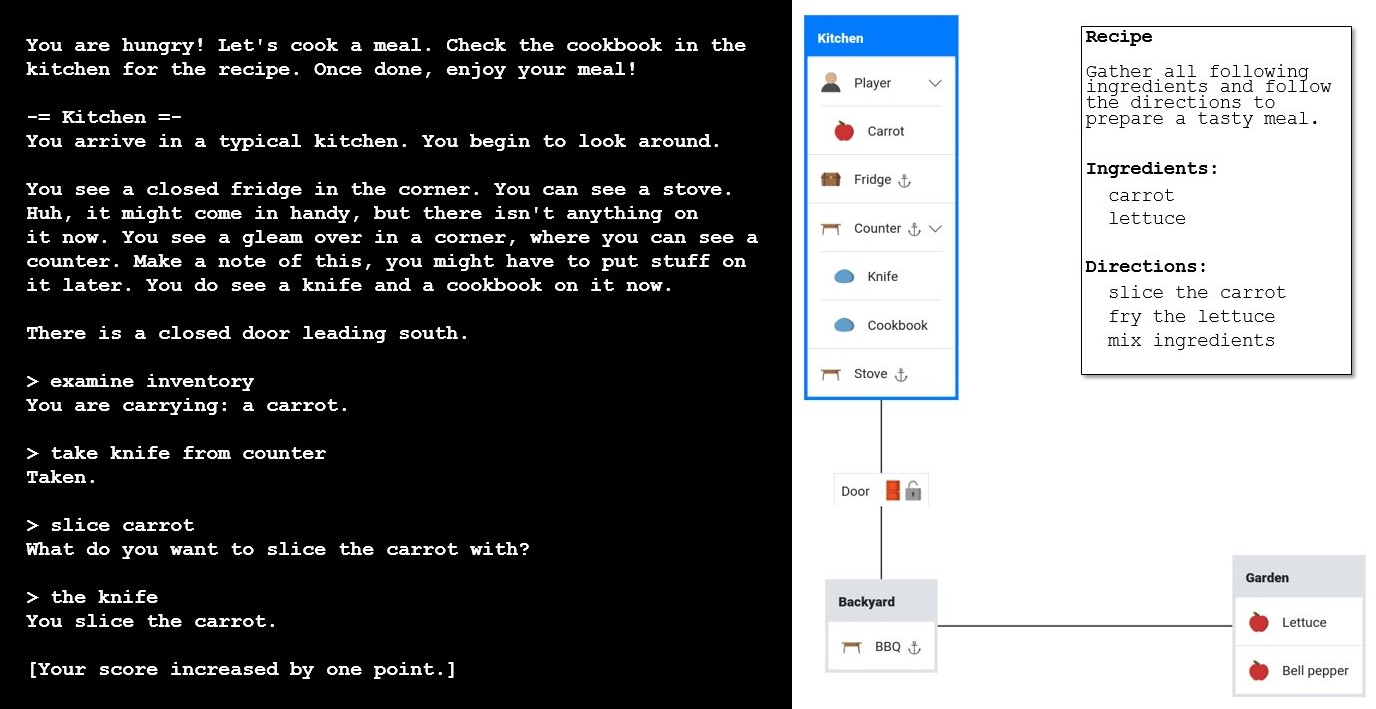
\includegraphics[width=1.0\textwidth]{iclr2025/images/textworld_map.png} 
    \caption{TextWorld interface along with visualization.}
    \label{fig:textworld_map} 
    \vspace{-2mm}
\end{figure}


\subsection{TextWorld Results}
In Table \ref{textworld_LLM}, we provide results for TextWorld. Standard errors are computed using 20 seeds for each of the 3 tasks. GPT-4o once again leads, obtaining more than twice the average progression of its closest competitor Llama 3.1 70B. The coin collector task was by far the most challenging, with GPT-4o managing to solve it only once out of 20 attempts. Gemini models' APIs often failed to return completions on textworld, flagging the inputs as "unsafe", despite there being absolutely no real safety concerns in the textworld gameplays. This made it impossible to complete a full round of evaluation on the Gemini models, thus we marked them as 0\% progression.

\begin{table}[h]
    \centering
    \begin{minipage}[t]{0.48\linewidth}
    \centering
    \caption{LLM Performance on textworld}
    \begin{tabular}{lc}
    \hline
    Model & Average Progress (\%) \\
    \hline
    claude-3.5-sonnet & 42.06 $\pm$ 5.41 \\
    gpt-4o & 39.31 $\pm$ 5.24 \\
    claude-3.5-haiku & 18.04 $\pm$ 5.81 \\
    llama-3.1-70b-it & 15.00 $\pm$ 4.61 \\
    gpt-4o-mini & 12.25 $\pm$ 3.55 \\
    llama-3.2-90b-it & 11.18 $\pm$ 2.98 \\
    llama-3.2-11b-it & 6.66 $\pm$ 2.17 \\
    llama-3.1-8b-it & 6.08 $\pm$ 2.41 \\
    llama-3.2-3b-it & 3.53 $\pm$ 1.06 \\
    llama-3.2-1b-it & 3.33 $\pm$ 0.91 \\
    gemini-1.5-flash & 0.00 $\pm$ 0.00 \\
    gemini-1.5-pro & 0.00 $\pm$ 0.00 \\
    \hline
    \label{textworld_LLM}
    \end{tabular}
    \end{minipage}
\end{table}

\subsection{Observations}


\env{You are an agent playing TextWorld, a text-based adventure game where you navigate through different
rooms, interact with objects, and solve puzzles.\newline\newline
Your goal is to first find the recipe, find and prepare food according to the recipe, and finally prepare and eat the meal.\newline\newline
Here are the available commands:\newline\newline
look: describe the current room \newline
goal: print the goal of this game\newline
inventory: print player's inventory \newline
go $<$dir$>$: move the player north, east, south or west.: move the player north, east, south or west. You can only go to directions indicated with an exit or a door. \newline
examine ...: examine something more closely\newline
eat ...: eat edible food \newline
open ...: open a door or a container. You need to open a closed door before you can go through
it. \newline
drop ...: drop an object onto the floor \newline
take ...: take an object that is visible \newline
put ... on ...: place an object on a supporter \newline
take ... from ...: take an object from a container or a supporter \newline
insert ... into ...: place an object into a container \newline
lock ... with ...: lock a door or a container with a key \newline
unlock ... with ...: unlock a door or a container with a key \newline
cook ... with ...: cook cookable food with something providing heat \newline
slice ... with ...: slice cuttable food with something sharp \newline
chop ... with ...: chop cuttable food with something sharp \newline
dice ... with ...: dice cuttable food with something sharp \newline
prepare meal: combine ingredients from inventory into a meal.\newline\newline You can only prepare meals in the Kitchen.\newline
- You can examine the cookbook to see the recipe when it is visible. \newline
- The BBQ is for grilling things, the stove is for frying things, the oven is for roasting things. Cooking ingredients in the wrong way will lead to a failure of the game. \newline
- Once you have got processed ingredients and the appropriate cooking tool ready, cook all of them according to the recipe. \newline
- There are two conditions to correctly cook something (grill/fry/roast): \newline
a) the ingredient you want to cook is in your inventory and \newline
b) there is a suitable cooking tool in the room, and then use 'cook . . . with . . . ' command. \newline
- When you need to chop/slice/dice ingredients, you need to take the knife and the ingredient in your inventory and then 'slice/chop/dice ... with knife' \newline
- Make sure to first process the food (chop/slice/dice) before you try to cook them. \newline
- When you have all the ingredients (that got processed or cooked according to the menu), you can 'prepare meal'
in the kitchen and then 'eat meal' to win the game. \newline
- The ingredients should EXACTLY match the color in the recipe, but if the recipe doesn't specify color, any color would be fine. When you 'take ... with ...', use the EXACT name you see. \newline
- You don't need to examine the container/supporter (e.g. toolbox) when it says something like "there isn't a thing on it"/"has nothing on it"\newline\newline
You have 80 steps to complete the task. Restarting is forbidden.
\newline\newline
PLAY!
}

\env{-= Street =-\newline
You find yourself in a street. An usual kind of place.\newline\newline
There is a closed sliding door leading north. There is an exit to the south.\newline\newline
-= Street =-0/1
}

\agent{open sliding door} 




